        %%******************************************%%
        %%                                          %%
        %%        Modello di tesi di laurea         %%
        %%            di Andrea Giraldin            %%
        %%                                          %%
        %%             2 novembre 2012              %%
        %%                                          %%
        %%******************************************%%

\begin{document}
    \frontmatter
    \begin{titlepage}
    \begin{center}
        \begin{LARGE}
            \textbf{\myUni}\\
        \end{LARGE}

        \vspace{10pt}

        \begin{Large}
            \textsc{\myDepartment}\\
        \end{Large}

        \vspace{10pt}

        \begin{large}
            \textsc{\myFaculty}\\
        \end{large}

        \vspace{30pt}
        \begin{figure}[htbp]
            \centering
            
\includegraphics[height=6cm]{unipd-logo}
        \end{figure}
        \vspace{30pt}

        \begin{LARGE}
            \textbf{\myTitle}\\
        \end{LARGE}

        \vspace{10pt}

        \begin{large}
            \textsl{\myDegree}\\
        \end{large}

        \vspace{40pt}

        \begin{large}
            \begin{flushleft}
                \textit{Relatore}\\
                \vspace{5pt}
                \profTitle\ \myProf
            \end{flushleft}

            % You can tweak the spacing to have professor and student names on the same line
            % useful if the page is broken by a long thesis title and you need more space
            % \vspace{-52pt}

            \begin{flushright}
                \textit{Laureando}\\
                \vspace{5pt}
                \myName
            \end{flushright}
        \end{large}

        \vspace{40pt}

        \line(1, 0){338} \\
        \begin{normalsize}
            \textsc{Anno Accademico \myAA}
        \end{normalsize}
    \end{center}
\end{titlepage}

    \clearpage
\phantomsection
\thispagestyle{empty}

\hfill
\vfill

\noindent\myName: \textit{\myTitle,}
\myDegree,
\textcopyright\ \myTime.

    % \cleardoublepage
\phantomsection
\thispagestyle{empty}
\pdfbookmark{Dedica}{Dedica}

\vspace*{3cm}

\begin{center}
    Lorem ipsum dolor sit amet, consectetuer adipiscing elit. \\ \medskip
    --- Oscar Wilde
\end{center}

\medskip

\begin{center}
    Dedicato a ...
\end{center}

    \cleardoublepage
\phantomsection
\pdfbookmark{Sommario}{Sommario}
\begingroup
\let\clearpage\relax
\let\cleardoublepage\relax
\let\cleardoublepage\relax

\chapter*{Sommario}

Il presente documento descrive il lavoro che ho svolto durante il periodo di \stage, della durata di trecentoventi ore, 
dal laureando {\myName} presso l'azienda {\azienda} \\
Gli obiettivi da raggiungere erano diversi.\\
In primo luogo era richiesto lo sviluppo di un \textit{plugin} Gradle per l'analisi statica delle dipendenze software di un progetto Gradle o npm;
in secondo luogo era richiesto di sviluppare dei servizi REST per il salvataggio dei risultati del \textit{plugin} e per effettuare la ricerca
delle vulnerabilità software note e, infine,
una \textit{web application} per la visualizzazione dei risultati.\\
Questo documento è strutturato in quattro capitoli principali:
\begin{enumerate}
    \item Il primo capitolo offre una panoramica del contesto aziendale e illustra gli strumenti utilizzati durante lo \stage.
    \item Nel secondo capitolo viene presentata la proposta di \stage, con un focus sugli obiettivi da raggiungere.
    \item Il terzo capitolo descrive in dettaglio le attività svolte durante lo \stage.
    \item Il quarto capitolo contiene riflessioni personali sull'esperienza lavorativa e sulle competenze acquisite.
\end{enumerate}

\noindent Durante la scrittura ho utilizzato termini in lingua inglese, in quanto è la lingua più utilizzata nel settore informatico, 
per riferirmi a concetti tecnici, essi sono stati evidenziati in \textit{corsivo}.\\
Per mettere in evidenza termini di particolare importanza ho utilizzato il \textbf{grassetto}.\\
Ho creato un glossario per chiarire il significativo di alcuni termini tecnici di non immediata comprensione, essi sono evidenziati in azzurro.\\
Ho allegato ad ogni figura un numero progressivo, in modo da poterla citare nel testo, ed una didascalia per descrivere il contenuto
e per citarne la fonte, se non è di mia creazione.\\


%\vfill

%\selectlanguage{english}
%\pdfbookmark{Abstract}{Abstract}
%\chapter*{Abstract}

%\selectlanguage{italian}

\endgroup

\vfill

    % \cleardoublepage
\phantomsection
\pdfbookmark{Ringraziamenti}{ringraziamenti}

% \begin{flushright}{
%     \slshape
%     ``Life is really simple, but we insist on making it complicated''} \\
%     \medskip
%     --- Confucius
% \end{flushright}


\bigskip

\begingroup
\let\clearpage\relax
\let\cleardoublepage\relax
\let\cleardoublepage\relax

\chapter*{Ringraziamenti}

\noindent \textit{Innanzitutto, vorrei esprimere la mia gratitudine al Prof. \myProf, relatore della mia tesi, per la pazienza, l'aiuto e il sostegno fornitomi durante la stesura del lavoro.}\\

\noindent \textit{Desidero ringraziare tutti quelli che mi sono stati vicini.}\\

\bigskip

\noindent\textit{\myLocation, \myTime}
\hfill \myName

\endgroup

    \cleardoublepage
\pdfbookmark{\contentsname}{tableofcontents}
\setcounter{tocdepth}{2}
\tableofcontents
%\markboth{\contentsname}{\contentsname}
\clearpage

\begingroup
    \let\clearpage\relax
    \let\cleardoublepage\relax
    \let\cleardoublepage\relax

    % Figures list
    \phantomsection
    \pdfbookmark{\listfigurename}{lof}
    \listoffigures

    \vspace*{8ex}

    % Tables list
    \phantomsection
    \pdfbookmark{\listtablename}{lot}
    \listoftables

    \vspace*{8ex}
    % Snippet list
    \phantomsection
    \pdfbookmark{Elenco dei frammendi di codice}{lot}
    \lstlistoflistings
    \vspace*{8ex}
  \endgroup

\cleardoublepage

    \cleardoublepage
    \mainmatter
    \chapter{L'azienda}
\label{cap:lazienda}


\section\azienda

\subsection{Descrizione}
L'azienda {\azienda}, fondata nel 1984, offre servizi di consulenza e sviluppo di software. 
Si è distinta nell'ideazione, costruzione e implementazione di strumenti software per oltre 2500 imprese, 
molte delle quali all'estero. \\
Una delle sue qualità distintive è l'attenzione verso i clienti, 
con vari uffici in regioni come Veneto, Lombardia, Emilia-Romagna, Friuli-Venezia Giulia, Toscana, Puglia e Campania, 
impiegando oltre 600 professionisti. \\
La sede centrale per la ricerca e sviluppo (CSV) si trova a Grisignano di Zocco (VI) e ospita più di 200 collaboratori. 
Qui, gruppi di sviluppatori 
e tecnici lavorano insieme per assicurare servizi affidabili e soluzioni software su misura. 
\newpage

\subsection{Organizzazione dell'azienza e i suoi prodotti}
{\azienda} è suddivisa in \textit{Business Unit} (BU), una parte di un'azienda che opera in modo autonomo o semi-autonomo, 
con la propria visione, \textit{mission}, obiettivi e strategie. Essa ha una propria \textit{leadership} e una struttura 
organizzativa separata, ed è responsabile del proprio profitto e perdite. \\
Le BU possono focalizzarsi su 
specifici mercati geografici, gruppi di clienti o linee di prodotti, permettendo all'azienda di essere 
più agile e rispondere meglio alle esigenze del mercato e dei clienti.\\
In {\azienda} BU sono 11 e, come rappresentate in figura \ref{fig:organizzazione-azienda}, si suddividono in:
\begin{itemize}
  \item \textbf{JGALILEO:} ha sviluppato l’\gls{ERP} –  Jgalileo, il sistema gestionale completo che consente alle imprese di monitorare e governare i flussi aziendali in modo semplice ed efficace, grazie a workflow condivisi e informazioni univoche e coerenti. Il software gestionale ERP Jgalileo si rivolge a tutte le aziende produttive e commerciali di ogni dimensione, dalla piccola azienda al grande gruppo aziendale internazionale, grazie anche alla gestione accurata delle fiscalità estere;
  \item \textbf{NEXTBI:} specializzata in \textit{Information Technology} e consulenza direzionale, con un focus nelle aree \textit{marketing}, vendite, \textit{retail}, \textit{customer innovation}, Business Intelligence, Corporate Performance Management e per le soluzioni \gls{IoT};
  \item \textbf{4WORDS:} specializzata in soluzioni \gls{B2B}, app e \gls{CRM}, ha l’obiettivo di far crescere le aziende grazie a soluzioni digitali dedicate: portale B2B, \gls{app} custom, app per la rete vendita e l’assistenza tecnica, ma anche realtà aumentata e \gls{PIM};
  \item \textbf{TCE:} si occupa di ottimizzare la fase di preventivazione e di acquisizione dell’ordine; \\
  Sviluppa il prodotto \gls{CPQg}, strumento essenziale ai fini della configurazione dell’offerta, 
  della gestione della trattativa e del recepimento del contratto, completo di tutti i contenuti documentali necessari.
  Attraverso uno strumento CPQ la forza vendite può configurare l’offerta più idonea in autonomia, in funzione delle specifiche esigenze del momento, senza preoccuparsi delle complesse logiche commerciali che la piattaforma gestisce in automatico;
  \item \textbf{DISCOVERY QUALITY:} produce una soluzione di Governance aziendale per gestire in modo efficace tutti i processi. 
  Un potente motore di workflow guida in modo preciso l’operatività del management e degli utenti, e inoltre misura le performance dell’impresa. \\
  Discovery Quality gestisce anche le principali normative internazionali e le metriche legate alla sostenibilità aziendale \gls{SDGs} e \gls{BCorp};
  \item \textbf{ECM:} propone le soluzioni software integrate ideali di \gls{ECM} per gestire al meglio i documenti digitali;
  \item \textbf{SMITECH:} si occupa di \gls{cybersecurity} e \gls{data_protection};
  \item \textbf{ELEMENT:} è la nuova divisione dedicata alla creazione di siti web ed e-commerce personalizzati, con una \textit{customer shopping experience} su misura;
  \item \textbf{JPA:} è il software di \gls{BPM} ideale per creare, gestire e automatizzare i processi aziendali integrandosi con qualsiasi sistema del cliente; gestendo automaticamente tutte le risorse;
  \item \textbf{FACTORY:} è la Business Unit che soddisfa tutte le necessità della \gls{Supply Chain} e delle fasi nella fabbrica del futuro;\\
  La suite di Factory è stata sviluppata per aumentare il livello di servizio ai clienti, ridurre i livelli di scorta di magazzino, ottimizzare l’utilizzo degli asset aziendali e massimizzare i profitti, riducendo i costi;
  \item \textbf{JPM:} è il software di \gls{Project Management} nato per supportare in modo semplice ed efficace le aziende nella gestione dei progetti, facilitando il raggiungimento degli obiettivi.

\end{itemize}


\begin{figure}[!h] 
  \centering 
  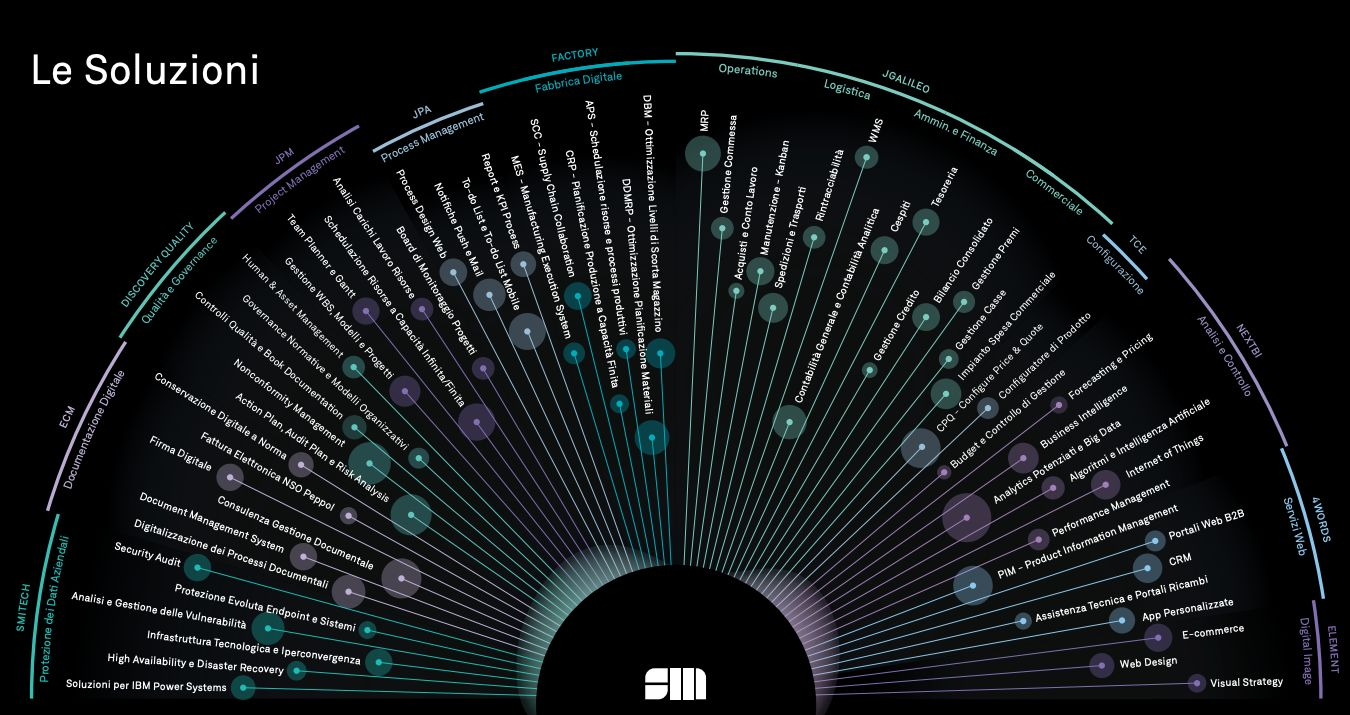
\includegraphics[width=1\columnwidth]{organizzazione-azienda} 
  \caption{Le BU di {\azienda} ed i loro prodotti}
  \label{fig:organizzazione-azienda}
\end{figure}

\noindent Ogni singola BU porta avanti diversi progetti ha un responsabile che si occupa di gestire il budget e le risorse umane. \\
Ogni progetto è formato da diverse figure:
\begin{itemize}
  \item Un \gls{PO} che si occupa di gestire il progetto e di interfacciarsi con il cliente;
  \item Uno \gls{Scrum Master} che si occupa di gestire il team di sviluppo e di facilitare il processo di sviluppo;
  \item Gli sviluppatori che si occupano di sviluppare il prodotto;
  \item I tester che si occupano di testare il prodotto;
  \item I consulenti che si occupano di interfacciarsi con il cliente, di capire le sue esigenze e successivamente di installare e configurare il prodotto;
  \item Gli \gls{analisti} che si occupano di analizzare i requisiti del cliente e di redigere la documentazione. Molte volte gli analisti sono anche sviluppatori e tester;
\end{itemize}

\noindent In aggiunta alle componenti precedentemente descritte, ci sono anche altre figure che compongono l'azienda:
\begin{itemize}
  \item \textbf{HR:} si occupa di gestire le risorse umane, di reclutare nuovi dipendenti e di gestire i rapporti con i dipendenti;
  \item \textbf{Marketing:} si occupa di gestire il sito web, i social network e di creare materiale pubblicitario;
  \item \textbf{Amministrazione:} si occupa di gestire la contabilità e le risorse economiche;
  \item \textbf{IT:} si occupa di gestire l'infrastruttura informatica e di fornire supporto ai dipendenti;
  \item \textbf{Commerciali:} si occupano di trovare nuovi clienti e di gestire i rapporti con i clienti esistenti;
  \item \textbf{Direzione:} si occupa di gestire l'azienda e di prendere decisioni strategiche;
  \item \textbf{Centralino:} si occupa di gestire le telefonate e di accogliere i clienti;
  \item \textbf{Presidente:} fondatore dell'azienda, si occupa di prendere decisioni strategiche e di gestire i rapporti con i clienti più importanti;
  \item \textbf{Amministratore delegato:} si occupa di gestire l'azienda e di prendere decisioni strategiche;
\end{itemize}

All'interno dell'azienda c'è una parte di dipendenti che lavora in sede, una parte che lavora in remoto e una parte che lavora presso i clienti. \\
Per riuscire a monitorare il lavoro di tutti i dipendenti, l'azienda utilizza un software di \textit{time tracking} che permette di registrare le ore lavorate. \\
Ogni dipendente ha un proprio \textit{account} che permette di registrare le ore lavorate, di richiedere ferie e permessi. \\
Il software permette di visualizzare le ore lavorate da ogni dipendente e di generare report per ogni progetto e per ogni cliente. \\
Durante l'inserimento delle ore lavorate (Rapporino), il dipendente deve inserire una descrizione delle attività svolte, la commessa, l'eventuale cliente,
la sede in cui ha lavorato, l'ora di inizio e fine lavoro ed eventualmente può collegare il Rapporino ad un ticket. \\
Questa operazione deve essere fatta per ogni giorno lavorativo e ad ogni chiusura del mese vengono bloccate le ore lavorate. \\

\newpage

\section{Il team di sviluppo}
Il team di sviluppo in cui ho lavorato fa parte della BU \textit{JPA} (\textit{Process Management}) e non si
occupa di sviluppare un prodotto specifico, ma ha come obiettivo quello di fornire supporto a tutti i team di sviluppo
dell'azienda. \\
Le principali attività del team sono le seguenti:
\begin{itemize}
  \item \textbf{Supporto:} il team fornisce supporto ai team di sviluppo per la risoluzione di problemi tecnici e analitici;
  \item \textbf{Formazione:} il team fornisce formazione ai team di sviluppo per l'utilizzo di nuovi strumenti e tecnologie;
  \item \textbf{Ricerca e sviluppo:} il team si occupa di sviluppare un \textit{\gls{frameworkg}} interno che permette di creare applicazioni web in modo semplice e veloce;
  \item \textbf{Automazione:} il team si occupa di automatizzare i processi di sviluppo, come ad esempio la compilazione, il rilascio di un prodotto o lo sviluppo di uno nuovo; 
  \item \textbf{Gestione repository:} il team si occupa di gestire i repository di codice sorgente e di fornire supporto per l'utilizzo di strumenti di \textit{\gls{continuous_integrationg}};
  \item \textbf{Installatore:} il team si occupa di sviluppare un installatore per i prodotti dell'azienda che utilizzano il \textit{\gls{frameworkg}} interno;
\end{itemize}

\noindent Il team è composto da 3 persone:
\begin{itemize}
  \item \textbf{Scrum Master:} si occupa di gestire il team e di prendere decisioni strategiche;
  \item \textbf{2 sviluppatori:} che si occupano di sviluppare il \textit{frameworkg} interno e di fornire supporto ai team di sviluppo;
\end{itemize}

Gli sviluppatori del team di sviluppo sono anche analisti e tester. \\


\section{Strumenti utilizzati}
I principali strumenti per lo sviluppo da me utilizzati sono stati i seguenti:\\
\begin{itemize}
  \item \textbf{Intellij IDEA:} un ambiente di sviluppo integrato (\gls{IDEg}) per il linguaggio di programmazione Java. Fornisce strumenti e funzionalità avanzate per supportare lo sviluppo efficiente del codice, il debug e la testing. Con la sua interfaccia user-friendly e le potenti funzionalità, come l'analisi statica del codice e il refactoring intelligente, IntelliJ IDEA è scelto da molti sviluppatori per creare applicazioni Java professionali;
  \item \textbf{WebStorm:} un IDE per lo sviluppo di applicazioni web, che fornisce un'esperienza di sviluppo ottimale. Grazie alla sua integrazione con strumenti di supporto per lo sviluppo web, come \textit{Node.js}, \textit{Angular}, \textit{React}, WebStorm permette di sviluppare applicazioni web moderne con facilità;
  \item \textbf{Neo4j Desktop:} un programma che permette di installare e gestire database \textit{Neo4j} in modo semplice e veloce. Permette di creare e gestire più database, di monitorare le performance e di eseguire query;
  \item \textbf{Git:} un sistema di controllo versione distribuito, utilizzato per il versionamento del codice sorgente; 
  \item \textbf{Gradle:} un sistema di automazione open source che gestisce le dipendenze e permette di automatizzare il processo di compilazione, testing, pubblicazione e deployment di un software;
  \item \textbf{Docker:} un progetto open source che automatizza il deployment di applicazioni all'interno di contenitori software, fornendo un'astrazione aggiuntiva grazie alla virtualizzazione a livello di sistema operativo di Linux;
  \item \textbf{Bitbucket:} un servizio di hosting per progetti che utilizzano Git come sistema di controllo versione. Fornisce strumenti per la collaborazione e la gestione del codice sorgente;
  \item \textbf{Jenkins:}  un software open source che permette di automatizzare il processo di \textit{build}, testing e deployment di un software;
  \item \textbf{Angular:} un {\gls{frameworkg}} open source per lo sviluppo di applicazioni web, scritto in TypeScript. 
  Fornisce un'architettura \gls{mvvm} e permette di creare applicazioni web dinamiche e scalabili;
  \item \textbf{Jira:} un software di tracciamento dei bug e gestione dei progetti, che permette di pianificare, monitorare e rilasciare software di qualità;
  \item \textbf{Confluence:} un software di collaborazione che permette di creare, organizzare e discutere documenti di progetto;
\end{itemize}

I linguaggi utilizzati sono i seguenti:\\

\begin{itemize}
  \item \textbf{Java:} un linguaggio di programmazione ad alto livello, orientato agli oggetti e a tipizzazione statica, che permette di creare applicazioni web, desktop e mobile;
  \item \textbf{Javascript:} un linguaggio di programmazione ad alto livello, orientato agli oggetti e a tipizzazione dinamica, che permette di creare applicazioni web dinamiche;
  \item \textbf{TypeScript:} un super-set di Javascript che permette di aggiungere tipizzazione statica al linguaggio;
  \item \textbf{Groovy:} un linguaggio di programmazione che permette di scrivere codice che viene eseguito sulla \gls{JVM};
  \item \textbf{Chyper:} un linguaggio di query dichiarativo per grafi, utilizzato per interrogare database \gls{Neo4j};
\end{itemize}

\subsection{Convenzioni}
Per lo sviluppo dei progetti che utilizzano il \textit{frameworkg} interno, sono state definite delle convenzioni da seguire.
Le convenzioni sono salvate all'interno di Confluence, in modo da essere facilmente accessibili a tutti i dipendenti. \\
Sono divise nelle seguenti categorie:
\begin{itemize}
  \item \textbf{Documentazione:} sono delle regole che indica come documentare il codice sorgente, in modo da facilitare la comprensione del codice;
  \item \textbf{Scrittura analisi:} sono delle regole che indicano come scrivere l'analisi dei requisiti e le strutture dell basi di dati, in modo da facilitare la comprensione dell'analisi;
  \item \textbf{Progettazione:} sono delle regole che indicano come progettare i componenti software, in modo da facilitare la manutenzione e l'estensione del codice;
  \item \textbf{Codifica:} sono delle regole che permettono di scrivere codice in modo uniforme, in modo da facilitare la lettura e la comprensione del codice;
  \item \textbf{Versionamento:} sono delle regole che indicano come versionare il codice sorgente, in modo da facilitare la gestione delle versioni;
\end{itemize}

\newpage
\section{Rapporto con l'innovazione}

{\azienda} ha come obiettivo l’innovazione delle aziende clienti per contribuire al loro progresso, 
agevolando la trasformazione digitale ed è specializzata nella progettazione e nella realizzazione di soluzioni integrate, 
a supporto della riorganizzazione di tutti i processi aziendali e professionali.\\
Per raggiungere questo obiettivo, l'azienda indirizza ogni anno dal 15 al 20\% del proprio fatturato all’attività di Ricerca e Sviluppo.\\
Uno dei punti di forza di {\azienda} è la capacità di cogliere le idee e i suggerimenti dei clienti, dei dipendenti, dei collaboratori e trarne ispirazione per sviluppare nuovi prodotti e nuove soluzioni
    \chapter{Il progetto di stage}
\label{cap:ilprogettodistage}

In questo capitolo descrivo il progetto di \textit{stage}, e le motivazioni che mi hanno spinto a scegliere questo progetto.\\
Ho scelto {\azienda} perchè è l'azienda per cui lavoro da più di 5 anni, e che mi ha dato la possibilità di crescere professionalmente.
Ho scelto questo progetto perchè mi ha permesso di lavorare con tecnologie nuove, e di imparare nuovi linguaggi di programmazione.\\
Lo \textit{stage} prevedeva lo sviluppo di un prototipo per il monitoraggio, la raccolta e l'analisi delle dipendenze \textit{software} degli applicativi di {\azienda}.\\
Il nome del progetto è \textit{Dependency Analyzer} ed è stato scelto dai membri del team di cui ho fatto parte.\\
\section{Lo \textit{stage} per \azienda}

Gli \textit{stage} rappresentano un pilastro fondamentale nella strategia di {\azienda}, svolgendo molteplici funzioni cruciali. 
Primo fra tutti, offrono l'opportunità di dedicarsi a progetti innovativi che, a causa di limitazioni di \textit{budget} o di tempo, 
non troverebbero spazio nelle attività lavorative ordinarie. I \textit{team} di sviluppo di {\azienda} sono primariamente impegnati 
nel mantenimento e nello sviluppo dei prodotti esistenti, lasciando poco margine per la ricerca e lo sviluppo di nuove idee. 
Questo compito solitamente è affidato al \textit{team} di ricerca e sviluppo, che, nonostante la sua competenza, è spesso limitato dalla scarsità 
di risorse umane per affrontare tutte le richieste innovative. In questo contesto, lo \textit{stage} diventa una soluzione efficace, 
consentendo lo sviluppo di prototipi e la conduzione di ricerche senza gravare eccessivamente sulle risorse aziendali.

L'investimento principale per l'azienda risiede nel tempo dedicato dal tutor aziendale alla guida e al supporto dello stagista. 
Pertanto, una selezione accurata sia del tutor sia dello stagista è essenziale per il successo del progetto e il raggiungimento 
degli obiettivi entro i tempi stabiliti.

\noindent Da anni, {\azienda} ha instaurato una proficua collaborazione con l'Università di Padova, accogliendo studenti per lo 
svolgimento di tesi di laurea e \textit{stage}. Questi periodi di formazione in azienda sono spesso orientati verso l'assunzione: negli 
ultimi anni, più di 140 stagisti sono entrati a far parte del team di {\azienda} a seguito del loro \textit{stage}.

Per lo studente, lo \textit{stage} si configura come un'esperienza formativa di grande valore. Consente di applicare concretamente le 
conoscenze teoriche acquisite durante il percorso di studi in un contesto lavorativo reale, favorendo al contempo l'acquisizione 
di nuove competenze e conoscenze. Questo periodo rappresenta un momento di verifica importante per lo studente, che ha l'opportunità 
di confrontarsi con il mondo del lavoro e di valutare se l'attività svolta corrisponde alle proprie aspettative e aspirazioni professionali future.


\section{La proposta di stage}

Un obiettivo strategico futuro per {\azienda} consiste nella modularizzazione dei propri prodotti \textit{software}. 
L'intento è quello di realizzare moduli che possano essere utilizzati in maniera autonoma e che, al contempo, 
siano facilmente integrabili con altre soluzioni. Questa direzione strategica implica un significativo aumento
del numero di progetti e delle interdipendenze tra essi, rendendo essenziale un'efficace gestione e monitoraggio di tali dipendenze.

In risposta a questa esigenza, il dipartimento di Ricerca e Sviluppo di {\azienda} ha intrapreso l'iniziativa 
di sviluppare un sistema avanzato per la raccolta, il monitoraggio e l'analisi delle dipendenze \textit{software}. 
L'obiettivo è quello di garantire un controllo accurato sulle versioni delle dipendenze collegate alle diverse release dei prodotti, 
contribuendo così a soddisfare i requisiti non funzionali in termini di sicurezza e affidabilità delle soluzioni offerte.

Nell'ambito di questa iniziativa, la proposta di \textit{stage} ha riguardato lo sviluppo di un \textit{\gls{prototipo}} per tale strumento. 
Il focus del progetto di \textit{stage} è stato lo sviluppo di un sistema in grado di raccogliere informazioni dettagliate sulle dipendenze 
direttamente dai sistemi di \textit{build} utilizzati per la compilazione dei prodotti, specificatamente \textit{\gls{Gradle}} e \textit{\gls{Npm}}. 
Questo prototipo rappresenta un passo fondamentale verso l'implementazione di una soluzione completa per la gestione delle dipendenze.

\subsubsection*{Il plugin \textit{Gradle}}
Il primo prodotto che l'azienda intendeva realizzare tramite lo \textit{stage} è un \textit{plugin} per \textit{Gradle} che raccoglie informazioni sulle dipendenze dei progetti java, 
analizzando l'albero delle dipendenze generato da \textit{Gradle}, e dei progetti \textit{npm} analizzandone il file \textit{package-lock.json} generato
durante l'installazione dei pacchetti.
Il plugin doveva poter essere pubblicato su un \textit{repository} interno aziendale, e doveva essere utilizzabile da tutti i progetti di {\azienda}.
Per essere più flessibile, doveva poter essere configurato specificando i nomi dei progetti \textit{npm} da analizzare
ed i riferimenti al \textit{backend} per l'invio delle informazioni raccolte.\\

\subsubsection*{Il backend}
Il secondo prodotto atteso era un \textit{backend} per il salvataggio e l'analisi delle informazioni raccolte. 
Il \textit{backend} doveva esporre dei servizi \textit{REST} per l'interrogazione del sistema, e doveva essere sviluppato utilizzando
il linguaggio di programmazione \textit{Java}. Non è stato richiesto l'utilizzo di un \textit{framework} specifico, ma è stato lasciata
la libertà di scegliere il \textit{framework} più adatto al progetto.\\
Il \textit{plugin} dopo aver raccolto le informazioni
le invia al \textit{backend} che,  dopo averle elaborate, le salva in un \textit{database} a grafo.
Anche in questo caso è stato richieso un file di configurazione per specificare i riferimenti al \textit{database} a grafo, e le credenziali
per l'autenticazione ai servizi \textit{REST}.\\

\subsubsection*{Il frontend}
Infine, un'interfaccia grafica realizzata tramite una \textit{web-app} per la visualizzazione delle informazioni raccolte.
Le specifiche per il \textit{frontend} erano molto generiche, ma per essere in linea con le tecnologie utilizzate in azienda,
è stato richiesto di utilizzare il \textit{framework Angular} per lo sviluppo.\\

\section{Obiettivi e aspettative}

\begin{figure}[!h] 
  \centering 
  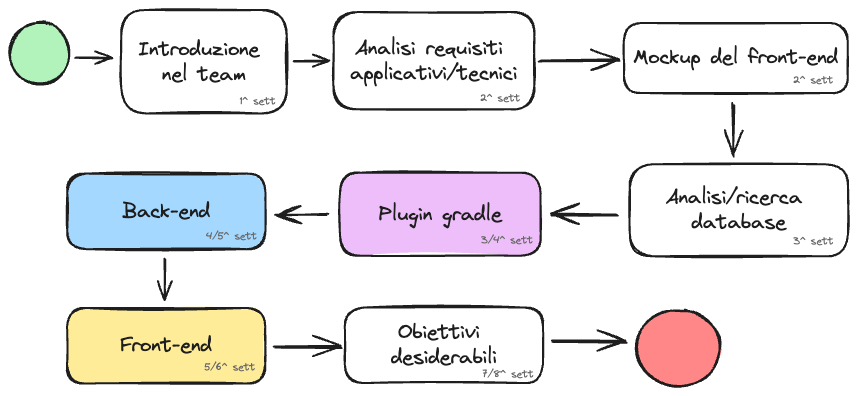
\includegraphics[width=1\columnwidth]{workflow-stage} 
  \caption{Sequenza temporale delle attività svolte durante lo \textit{stage}.}
  \label{fig:workflow-stage}
\end{figure}

L'identificazione degli obiettivi e delle aspettative è un passo fondamentale per la definizione di un progetto di \textit{stage}.
In questo contesto, gli obiettivi rappresentano le funzionalità che il sistema deve implementare, mentre le aspettative
sono le caratteristiche che il sistema deve possedere.\\
Gli obiettivi e le aspettative del progetto di \textit{stage} sono stati definiti in collaborazione con il tutor aziendale, 
tramite il piano di lavoro.
Esso è stato redatto prima dell'inizio dello \textit{stage}, e ha rappresentato un punto di riferimento per la valutazione
delle attività svolte durante il periodo di \textit{stage}.\\
All'interno del piano di lavoro erano presenti obiettivi obbligatori e obiettivi desiderabili.
Gli obiettivi avevano un codice identificativo, e una descrizione.\\ 
Il codice identificativo era composto da una lettera che rappresentava la tipologia di obiettivo, e da un numero progressivo.
Il progressivo ha permesso l'ordinamento, non casuale, degli obiettivi. \\
La pianificazione settimanale scritta nel piano di lavoro è stata una vera e propria guida per lo svolgimento delle attività, ed 
ha permesso di rispettare le scadenze, raggiungendo gli obiettivi prefissati in ordine di priorità, portando quelli desiderabili
a termine solo se il tempo lo permetteva.\\

Nel piano di lavoro gli obiettivi non erano molto dettagliati, questo ci ha permesso di avere una certa flessibilità durante lo svolgimento
delle attività, e di poter cambiare gli obiettivi in corso d'opera, se necessario.\\

\begin{table}[!h]
  \caption{Obiettivi obbligatori}
  \label{tab:obiettivi-obbligatori}
\begin{tabularx}{\textwidth}{lX}
   \textbf{Identificativo}&\textbf{Descrizione}\\ 
    \hline O01&Analisi dell'attuale infrastruttura\\
    \hline O02&Analisi requisiti applicativi e tecnici e \textit{mockup} del \textit{front end}\\
    \hline O03&Identificazione del db a grafo più adeguato al progetto\\
    \hline O04&Implementazione della struttura di \textit{database}\\
    \hline O05&Implementazione di un \textit{plugin gradle} per la raccolta delle informazioni\\
    \hline O06&Invocazione da \textit{jenkins}\\
    \hline O07&Implementazione dei servizi \textit{backend} per l'interrogazione del sistema\\
    \hline O08&Implementazione del \textit{front end} per rendere possibile l'interrogazione\\
    \hline 
\end{tabularx}
\end{table}

  \begin{table}[!h]
    \caption{Obiettivi desiderabili}
    \label{tab:obiettivi-desiderabili}
    \begin{tabularx}{\textwidth}{lX}
    \textbf{Identificativo}&\textbf{Descrizione}\\ 
    \hline D01&Possibilità di visualizzare i risultati in forma grafica (grafo) e non solo tabellari\\
    \hline D02&Integrazione con \textit{repository} remoti al fine di verificare nuove versioni delle dipendenze\\
    \hline D03&Integrazione con \textit{repository} remoti al fine di identificare vulnerabilità sulle dipendenze utilizzate\\
    \hline D04&Login con \textit{LDAP} aziendale\\  
    \hline
  \end{tabularx}
  \end{table}



  \section{Vincoli}
  \subsection*{ Vincoli tecnologici}

  Il piano di lavoro tramite gli obiettivi, intrinsecamente, ha definito i vincoli tecnologici del progetto.\\
  Il primo vincolo è stato quello di utilizzare un \textit{database} a grafo per il salvataggio dei dati raccolti dal \textit{plugin},
  questo perchè permette di rappresentare le dipendenze in maniera naturale, e di eseguire \textit{query} molto complesse in tempi molto brevi.\\
  Con i membri del team abbiamo deciso di utilizzare \textit{Neo4j} come \textit{database} a grafo, perchè è il più utilizzato, ha una comunità molto attiva
ed è molto ben documentato.

Il secondo vincolo tecnologico è stato quello di utilizzare \textit{Gradle} per il \textit{plugin} che raccoglie le informazioni sulle dipendenze,
questo perchè quasi tutti i progetti di {\azienda} lo utilizzano come sistema di build.\\

\subsubsection*{Gralde}
  \textit{Gradle} è uno strumento di automazione della \textit{build} \textit{open source} che si è guadagnato una notevole popolarità nel mondo 
dello sviluppo \textit{software}, grazie alla sua flessibilità e potenza. Utilizzato principalmente per progetti \textit{Java}, 
è anche ampiamente adottato per applicazioni scritte in altri linguaggi di programmazione come \textit{Kotlin}, \textit{C++}, e \textit{Python}. 
La sua caratteristica principale è la capacità di supportare configurazioni di \textit{build} altamente personalizzabili, 
rendendolo adatto sia per piccoli progetti sia per grandi imprese con esigenze complesse.

\textit{Gradle} si distingue per l'uso di un \gls{DSLg} basato sui linguaggi di programmazione \textit{Groovy} o \textit{Kotlin},
 che fornisce un modo intuitivo e dichiarativo di definire le \textit{build}. Questo approccio, combinato con la sua potente capacità di 
 gestione delle dipendenze e il suo modello di esecuzione incrementale, consente agli sviluppatori di costruire \textit{software} in modo più 
 efficiente e affidabile. Inoltre, \textit{Gradle} è noto per la sua velocità, superando spesso altri strumenti di \textit{build} come \textit{Maven} 
 e \textit{Ant}, specialmente in progetti di grandi dimensioni.

 \begin{figure}[!h] 
  \centering 
  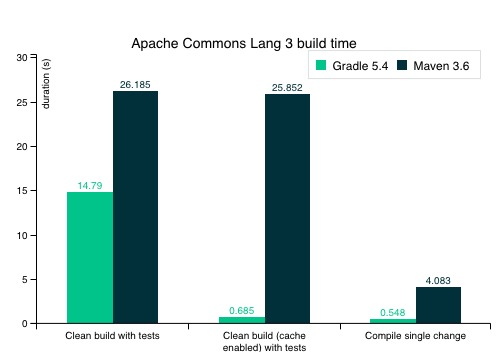
\includegraphics[width=1\columnwidth]{gradle-vs-maven.jpeg} 
  \caption{Comparazione tra \textit{Gradle} e \textit{Maven}. Fonte: https://gradle.org/maven-vs-gradle}
  \label{fig:gredle-vs-maven}
\end{figure}

Un altro aspetto fondamentale di \textit{Gradle} è la sua estensibilità. Gli sviluppatori possono estendere le funzionalità di \textit{Gradle} 
scrivendo script personalizzati o integrando \textit{plugin} esistenti. Questa flessibilità lo rende uno strumento ideale per adattarsi a 
flussi di lavoro specifici e requisiti di \textit{build} unici. Gradle è anche il sistema di \textit{build} ufficiale per \textit{Android}, ulteriormente 
consolidando la sua posizione come uno strumento chiave nello sviluppo di applicazioni moderne.

\subsubsection*{\textit{Angular}}
Un altro vincolo tecnologico è stato quello di utilizzare \textit{Angular} per lo sviluppo del \textit{frontend}, 
questo perchè, come scritto precedentemente, è il \textit{framework} più utilizzato in azienda per lo sviluppo delle \textit{web-app}.\\

\textit{Angular} è un \textit{framework} \textit{front-end} \textit{open source} sviluppato e mantenuto da \textit{Google}. 
È ampiamente riconosciuto per la sua capacità di creare applicazioni \textit{web} dinamiche e reattive. 
\textit{Angular} utilizza \textit{TypeScript}, una \textit{super-set} di \textit{JavaScript}, che fornisce funzionalità di tipizzazione statica e 
orientamento agli oggetti, migliorando la manutenibilità e la qualità del codice.

Una delle caratteristiche distintive di \textit{Angular} è il suo approccio basato su componenti, che aiuta gli sviluppatori a 
costruire applicazioni \textit{web} complesse in modo più modulare e mantenibile. Ogni componente in \textit{Angular} è una combinazione di \textit{HTML}, 
\textit{CSS}, e \textit{TypeScript}, che gestisce una parte specifica dell'interfaccia utente. Questo approccio promuove la riusabilità 
del codice e una migliore separazione delle preoccupazioni.

\textit{Angular} è anche noto per il suo potente sistema di \textit{dependency injection}, che semplifica lo sviluppo e il \textit{testing} fornendo un 
modo per iniettare dipendenze in classi in modo pulito e flessibile. Inoltre, \textit{Angular} offre un'ampia gamma di funzionalità integrate come il 
\textit{routing}, la gestione delle \textit{form}, e l'accesso HTTP, che accelerano lo sviluppo di applicazioni textit{web}.

\begin{figure}[h] 
  \centering 
  
\includegraphics[width=0.5\columnwidth]{feature-angular.png} 
  \caption{Caratteristiche di \textit{Angular}.}
  \label{fig:workflow-stage}
\end{figure}

Con il suo ecosistema ricco e una forte comunità di sviluppatori, \textit{Angular} è diventato uno dei \textit{framework} \textit{front-end} più popolari e 
affidabili per lo sviluppo di applicazioni \textit{web} moderne, sia per progetti di piccole dimensioni sia per applicazioni aziendali di grande scala.

\subsubsection*{I database a grafo e \textit{Neo4j}}

I \textit{database} a grafo sono una categoria di \textit{database} NoSQL progettati per gestire e rappresentare dati complessi e le loro relazioni 
in modo più efficiente rispetto ai tradizionali \textit{database} relazionali. Questi \textit{database} utilizzano strutture di grafo per la memorizzazione 
semantica, con nodi, bordi e proprietà per rappresentare e memorizzare dati. La flessibilità dei \textit{database} a grafo li rende particolarmente 
adatti per applicazioni che richiedono l'analisi di relazioni complesse e interconnesse, come i \textit{social network}, i sistemi di raccomandazione, 
e la gestione delle reti.

\textit{Neo4j} è uno dei più popolari \textit{database} a grafo, noto per la sua alta \textit{performance} e flessibilità. È un \textit{database} \textit{open source}, 
ma offre anche una versione \textit{enterprise} con funzionalità aggiuntive. \textit{Neo4j} utilizza il linguaggio di \textit{query} \textit{Cypher}, che è specificamente 
progettato per lavorare con grafi. \textit{Cypher} consente agli sviluppatori di esprimere facilmente \textit{query} complesse sulle relazioni tra i dati, 
rendendo \textit{Neo4j} particolarmente potente per analisi di dati relazionali complessi.

\begin{figure}[h] 
  \centering 
  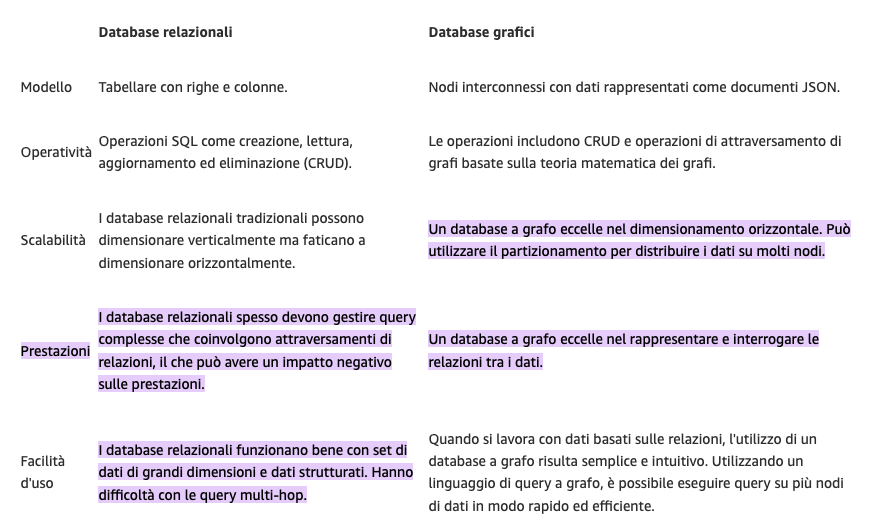
\includegraphics[width=1\columnwidth]{graphdb-vs-sql.png} 
  \caption{Differenze tra \textit{database} a grafo e \textit{database} relazionali. \\Fonte: https://aws.amazon.com/it/compare/the-difference-between-graph-and-relational-database.}
  \label{fig:graphdb-vs-sql}
\end{figure}

\subsection*{ Vincoli di dominio}
Il proddotto finale dovrà essere utilizzato, non solo dagli sviluppatori, ma anche dai \textit{project manager}, i \textit{team leader}, e i \textit{product owner} ed
i consulenti; Per questo è stato richiesto, come obiettivo desiderabile, di implementare l'autenticazione tramite \textit{LDAP} aziendale, 
per permettere l'accesso a tutti i dipendenti di {\azienda}.\\
L'\textit{LDAP} è un protocollo di rete che permette la gestione centralizzata delle autenticazioni e delle autorizzazioni.
Questo è fondamentale per garantire la sicurezza dei dati, e per permettere l'accesso solo a chi ne ha i permessi, senza dover
implementare un sistema di autenticazione ad hoc.\\



\section{La scelta dello stage}
La scelta dello stage non è stata molto semplice. La scelta principale da fare era, se scegliere un progetto interno all'azienda, o 
se momentaneamente abbandonare l'azienda per fare l'esperienza di stage in un'altra azienda.\\ 
Lo stage per me rappresenta un'opportunità per imparare nuove tecnologie, e per mettermi alla prova in un ambiente lavorativo diverso 
e questa poteva essere l'occasione giusta. Dopo aver valutato i pro e i contro, ho deciso di rimanere in azienda, perchè siamo riusciti
a trovare un progetto molto interessante e stimolante, che mi ha permesso di imparare nuove tecnologie, e di mettermi alla prova.\\

Questo progetto avrebbe permesso di affrontare problemi riguardanti lo sviluppo \textit{software}, problemi di gestione e organizzazione del lavoro ma 
anche i problemi riguardanti i sistemi di \textit{build} e di \textit{continuous integration}, un argomento che mi ha sempre affascinato ma che non ho mai
avuto modo di approfondire.\\

\section{Pianificazione e interazioni con il tutor}
All'inizio dello \textit{stage} ho avuto un incontro con il tutor aziendale, per discutere del piano di lavoro, e per definire la modalità
di svoldimento e di interazione durante lo \textit{stage}.\\
Abbiamo deciso di fare un incontro settimanale, per discutere delle attività svolte durante la settimana, e per pianificare le attività
della settimana successiva.\\
Quando avevo dei dubbi o dei problemi, potevo contattarelo tramite \textit{Google Chat} o tramite \textit{email}.\\
Ogni mattina alle 9:00 avevamo un incontro con il \textit{team} di sviluppo, per discutere delle attività svolte il giorno precedente, e per
pianificare le attività della giornata, come previsto dalla metodologia \textit{Agile}.\\
A questo incontro non partecipava il tutor aziendale. 
Capitava spesso comunque di avere degli incontri al di fuori di quelli pianificati, per discutere di problemi, principalmente analitici, 
e per prendere decisioni riguardanti l'implementazione.\\

\begin{figure}[h] 
  \centering 
  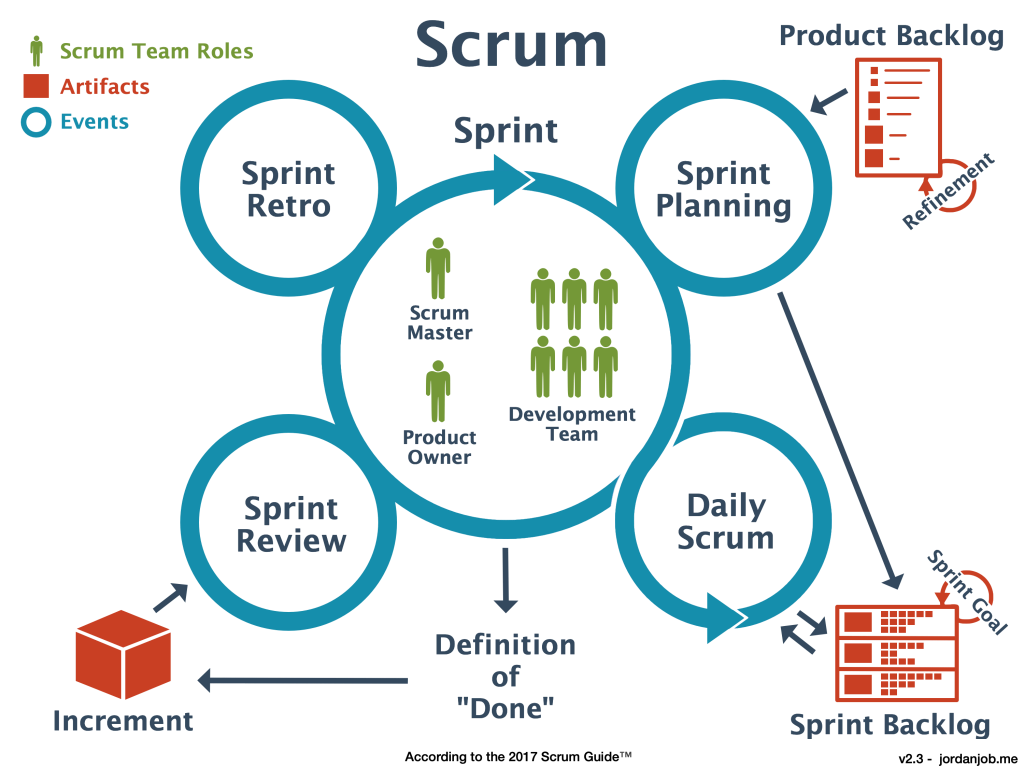
\includegraphics[width=.8\columnwidth]{scrum_agile.png} 
  \caption{Metodologia \textit{Agile}. Fonte: https://jordanjob.me/blog/scrum-diagram. }
  \label{fig:scrum_agile}
\end{figure}

    \appendix
    \chapter{Appendice A}

\epigraph{Citazione}{Autore della citazione}


    \backmatter
    \printglossary[type=\acronymtype, title=Acronimi e abbreviazioni, toctitle=Acronimi e abbreviazioni]
    \printglossary[type=main, title=Glossario, toctitle=Glossario]

    \cleardoublepage
\chapter{Bibliografia}

\nocite{*}

% Print book bibliography
\printbibliography[heading=subbibliography,title={Riferimenti bibliografici},type=book]

% Print site bibliography
\printbibliography[heading=subbibliography,title={Siti web consultati},type=online]

\end{document}
